% Auteur : Samuele Giraudo
% Création : oct. 2013
% Modifications : août 2014, oct. 2014, déc. 2015

\tikzstyle{Case}=[rectangle,draw=black,line width=1pt, minimum size=2cm,
minimum height=1cm]
\tikzstyle{Bloc}=[rectangle,draw=Vert!100,fill=Vert!20,
    line width=1pt,minimum width=1cm,minimum height=0.75cm]
\tikzstyle{BlocM}=[Bloc,draw=Marron=!100,fill=Marron!10]

%%%%%%%%%%%%%%%%%%%%%%%%%%%%%%%%%%%%%%%%%%%%%%%%%%%%%%%%%%%%%%%%%%%%%%%%
%%%%%%%%%%%%%%%%%%%%%%%%%%%%%%%%%%%%%%%%%%%%%%%%%%%%%%%%%%%%%%%%%%%%%%%%
%%%%%%%%%%%%%%%%%%%%%%%%%%%%%%%%%%%%%%%%%%%%%%%%%%%%%%%%%%%%%%%%%%%%%%%%
\section{Allocation dynamique}

%%%%%%%%%%%%%%%%%%%%%%%%%%%%%%%%%%%%%%%%%%%%%%%%%%%%%%%%%%%%%%%%%%%%%%%%
%%%%%%%%%%%%%%%%%%%%%%%%%%%%%%%%%%%%%%%%%%%%%%%%%%%%%%%%%%%%%%%%%%%%%%%%
\subsection{Pointeurs}

%%%%%%%%%%%%%%%%%%%%%%%%%%%%%%%%%%%%%%%%%%%%%%%%%%%%%%%%%%%%%%%%%%%%%%%%
\begin{frame} \frametitle{La mémoire}
Lors de l'exécution d'un programme, une portion (de taille variable) de
la mémoire lui est dédiée. Cette zone lui est exclusive. On l'appelle
la \alert{mémoire}.
\medskip

\uncover<2->{
On peut voir la mémoire comme un {\bf très grand tableau d'octets}.}

\uncover<3->{
\begin{multicols}{2} \small
La mémoire est segmentée en plusieurs parties~:
\begin{itemize}
    \item la {\bf zone statique} qui contient le code et les
    données statiques~;
    \item le {\bf tas}, de taille variable au fil de l'exécution~;
    \item la {\bf pile}, de taille variable au fil de l'exécution.
\end{itemize}
Il y a d'autres zones (non repr. ici).
\begin{center}
\scalebox{.6}{\begin{tikzpicture}
    \node[Zone,fill=Rouge!30](1)at(0,0){Zone statique};
    \node[Zone,fill=Bleu!30](2)at(0,-1.5){Tas\phantom{q}};
    \node[Zone,fill=Vert!30](3)at(0,-3){\dots\phantom{Tq}};
    \node[Zone,fill=Marron!30](4)at(0,-4.5){Pile\phantom{q}};
    \node[Zone,fill=gray!30,minimum height=.5cm](5)at(0,-5.5){Autre\phantom{q}};
    \draw[->,line width=1.5pt](-2,-1.5)--(-2,-2.5);
    \draw[->,line width=1.5pt](-2,-4.5)--(-2,-3.5);
\end{tikzpicture}}
\end{center}
\end{multicols}}
\medskip

\uncover<4->{
Le tas contient les variables allouées dynamiquement.
\medskip

La pile contient les variables locales lors des appels aux fonctions.}
\end{frame}

%%%%%%%%%%%%%%%%%%%%%%%%%%%%%%%%%%%%%%%%%%%%%%%%%%%%%%%%%%%%%%%%%%%%%%%%
\begin{frame} \frametitle{Pointeurs}
Nous avons vu que chaque variable possède une \alert{adresse}.
\bigskip

Connaître l'adresse d'une variable est suffisant pour la manipuler
(c.-à-d., lire et modifier sa valeur). L'objet qui permet de représenter
et de manipuler des adresses est le \alert{pointeur}.
\bigskip

\uncover<2->{
Un \alert{pointeur} est une entité constituée des deux éléments suivants~:

\begin{enumerate}
    \item une adresse vers une zone de la mémoire~;
    \smallskip
    
    \item un type.
\end{enumerate}}
\end{frame}

%%%%%%%%%%%%%%%%%%%%%%%%%%%%%%%%%%%%%%%%%%%%%%%%%%%%%%%%%%%%%%%%%%%%%%%%
\begin{frame} \frametitle{Pointeurs}
{\bf Intuitivement}, un pointeur est une \alert{flèche} munie d'un mode 
d'emploi, le tout pointant vers une zone de la mémoire.
\smallskip

Le \alert{mode d'emploi} décrit le type de la zone de la mémoire ainsi 
adressée en renseignant sur la taille de la zone.
\medskip

\begin{multicols}{2}
\uncover<2->{Si \Code{ptr\_1} est un pointeur sur une donnée de type 
\Code{int} ($4$ octets)~:
\begin{center}
    \scalebox{.5}{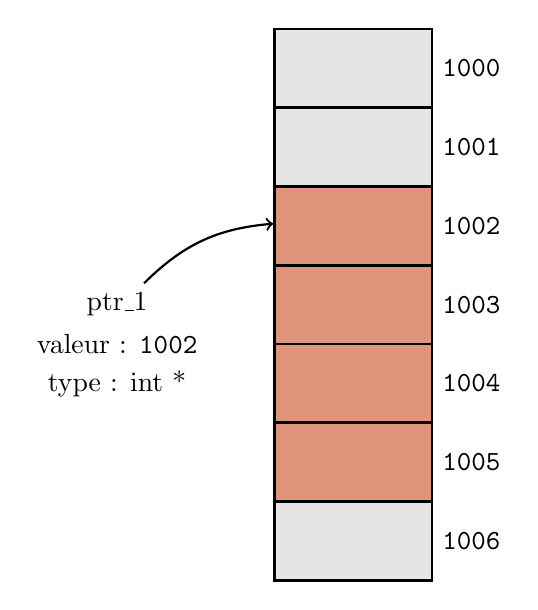
\begin{tikzpicture}
        \node[Case,fill=Gray!20](1)at(0,-1){};
        \node[Case,fill=Gray!20](2)at(0,-2){};
        \node[Case,fill=BrickRed!40](3)at(0,-3){};
        \node[Case,fill=BrickRed!40](4)at(0,-4){};
        \node[Case,fill=BrickRed!40](5)at(0,-5){};
        \node[Case,fill=BrickRed!40](6)at(0,-6){};
        \node[Case,fill=Gray!20](7)at(0,-7){};
        \node[right of=1,node distance=1.5cm]{\tt 1000};
        \node[right of=2,node distance=1.5cm]{\tt 1001};
        \node[right of=3,node distance=1.5cm]{\tt 1002};
        \node[right of=4,node distance=1.5cm]{\tt 1003};
        \node[right of=5,node distance=1.5cm]{\tt 1004};
        \node[right of=6,node distance=1.5cm]{\tt 1005};
        \node[right of=7,node distance=1.5cm]{\tt 1006};
        \node(p)at(-3,-4){\Code{ptr\_1}};
        \draw(p)edge[thick,->,bend right=-20](3);
        \node(p_val)at(-3,-4.5){valeur : {\tt 1002}};
        \node(p_type)at(-3,-5){type : \Code{int *}};
    \end{tikzpicture}}
\end{center}}

\uncover<3->{Si \Code{ptr\_2} est un pointeur sur une donnée de type 
\Code{char} ($2$ octets)~:
\begin{center}
    \scalebox{.5}{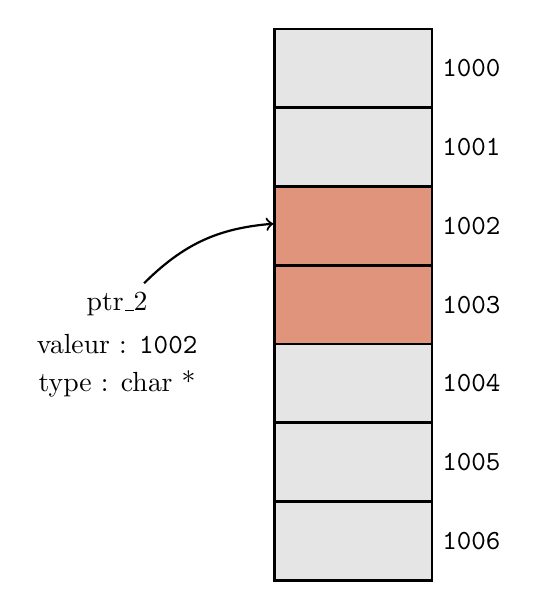
\begin{tikzpicture}
        \node[Case,fill=Gray!20](1)at(0,-1){};
        \node[Case,fill=Gray!20](2)at(0,-2){};
        \node[Case,fill=BrickRed!40](3)at(0,-3){};
        \node[Case,fill=BrickRed!40](4)at(0,-4){};
        \node[Case,fill=Gray!20](5)at(0,-5){};
        \node[Case,fill=Gray!20](6)at(0,-6){};
        \node[Case,fill=Gray!20](7)at(0,-7){};
        \node[right of=1,node distance=1.5cm]{\tt 1000};
        \node[right of=2,node distance=1.5cm]{\tt 1001};
        \node[right of=3,node distance=1.5cm]{\tt 1002};
        \node[right of=4,node distance=1.5cm]{\tt 1003};
        \node[right of=5,node distance=1.5cm]{\tt 1004};
        \node[right of=6,node distance=1.5cm]{\tt 1005};
        \node[right of=7,node distance=1.5cm]{\tt 1006};
        \node(p)at(-3,-4){\Code{ptr\_2}};
        \draw(p)edge[thick,->,bend right=-20](3);
        \node(p_val)at(-3,-4.5){valeur : {\tt 1002}};
        \node(p_type)at(-3,-5){type : \Code{char *}};
    \end{tikzpicture}}
\end{center}}
\end{multicols}
\end{frame}

%%%%%%%%%%%%%%%%%%%%%%%%%%%%%%%%%%%%%%%%%%%%%%%%%%%%%%%%%%%%%%%%%%%%%%%%
\begin{frame} \frametitle{Déclaration de pointeurs}
On \alert{déclare} un pointeur sur une zone de la mémoire de type \Code{T} par
\begin{center} \Code{T *ptr;} \end{center}
\medskip

\uncover<2->{
On \alert{accède à la valeur} de la zone mémoire pointée par \Code{ptr}
par
\begin{center} \Code{*ptr} \end{center}}

\uncover<3->{
On \alert{accède à l'adresse} de la zone mémoire pointée par \Code{ptr} par
\begin{center} \Code{ptr} \end{center}
\bigskip}

\uncover<4->{
{\bf Attention}~: le même symbole \Code{'*'} est utilisé pour la
déclaration d'un pointeur et pour accéder à la valeur pointée.
C'est une imperfection du langage {\sf C} qui peut porter à confusion.}
\end{frame}

%%%%%%%%%%%%%%%%%%%%%%%%%%%%%%%%%%%%%%%%%%%%%%%%%%%%%%%%%%%%%%%%%%%%%%%%
\begin{frame} \frametitle{Manipulation de pointeurs}
On suppose que \Code{ptr} est un pointeur pointant sur une zone de la
mémoire de type \Code{T}.
\bigskip
\bigskip

\uncover<2->{
Il est possible de \alert{changer l'endroit} où \Code{ptr} pointe par
\begin{center} \Code{ptr = ADR;} \end{center}
où \Code{ADR} est une adresse de la mémoire de type \Code{T}.
\bigskip
\bigskip}

\uncover<3->{
Il est possible d'\alert{affecter une valeur} \Code{VAL} de type \Code{T}
à \Code{*ptr} par
\begin{center} \Code{*ptr = VAL;} \end{center}
De cette manière, la zone mémoire d'adresse \Code{ptr} est modifiée et
devient de valeur \Code{VAL}.}
\end{frame}

%%%%%%%%%%%%%%%%%%%%%%%%%%%%%%%%%%%%%%%%%%%%%%%%%%%%%%%%%%%%%%%%%%%%%%%%
\begin{frame}[fragile] \frametitle{Manipulation de pointeurs --- exemple}
\begin{multicols}{2}
\begin{lstlisting}
/* (1) */
int num1, num2;
int *ptr1, *ptr2;
num1 = 10;
num2 = 20;

/* (2) */
ptr1 = &num1;
ptr2 = &num2;
*ptr1 = 100;
*ptr2 = 200;

/* (3) */
ptr2 = ptr1;
*ptr1 = 300;
*ptr2 = 400;
\end{lstlisting}

\scalebox{.6}{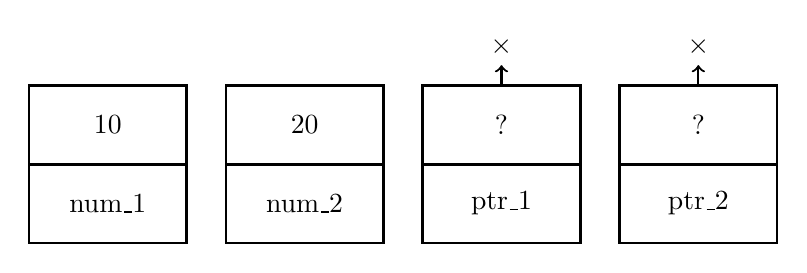
\begin{tikzpicture}
    \node[Case](num_1_nom)at(0,0){\Code{num\_1}};
    \node[Case](num_1_val)at(0,1){\Code{10}};
    %
    \node[Case](num_2_nom)at(2.5,0){\Code{num\_2}};
    \node[Case](num_2_val)at(2.5,1){\Code{20}};
    %
    \node[Case](ptr_1_nom)at(5,0){\Code{ptr\_1}};
    \node[Case](ptr_1_val)at(5,1){\Code{?}};
    \node(croix_1)at(5,2){\begin{math}\times\end{math}};
    \draw(ptr_1_val)edge[thick,->](croix_1);
    %
    \node[Case](ptr_2_nom)at(7.5,0){\Code{ptr\_2}};
    \node[Case](ptr_2_val)at(7.5,1){\Code{?}};
    \node(croix_2)at(7.5,2){\begin{math}\times\end{math}};
    \draw(ptr_2_val)edge[thick,->](croix_2);
\end{tikzpicture}}

\scalebox{.6}{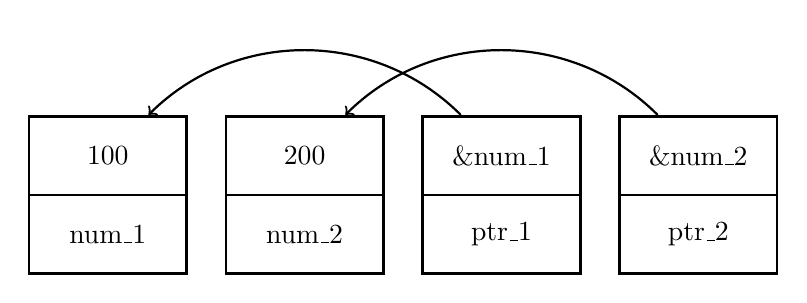
\begin{tikzpicture}
    \node[Case](num_1_nom)at(0,0){\Code{num\_1}};
    \node[Case](num_1_val)at(0,1){\Code{100}};
    %
    \node[Case](num_2_nom)at(2.5,0){\Code{num\_2}};
    \node[Case](num_2_val)at(2.5,1){\Code{200}};
    %
    \node[Case](ptr_1_nom)at(5,0){\Code{ptr\_1}};
    \node[Case](ptr_1_val)at(5,1){\Code{\&num\_1}};
    \draw(ptr_1_val)edge[thick,->,bend right=45](num_1_val);
    %
    \node[Case](ptr_2_nom)at(7.5,0){\Code{ptr\_2}};
    \node[Case](ptr_2_val)at(7.5,1){\Code{\&num\_2}};
    \draw(ptr_2_val)edge[thick,->,bend right=45](num_2_val);
\end{tikzpicture}}

\scalebox{.6}{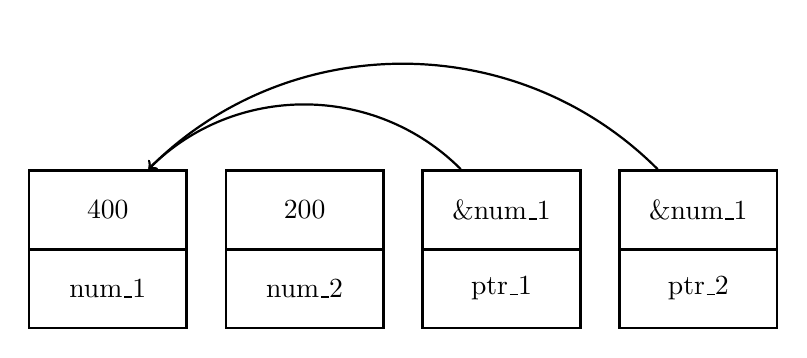
\begin{tikzpicture}
    \node[Case](num_1_nom)at(0,0){\Code{num\_1}};
    \node[Case](num_1_val)at(0,1){\Code{400}};
    %
    \node[Case](num_2_nom)at(2.5,0){\Code{num\_2}};
    \node[Case](num_2_val)at(2.5,1){\Code{200}};
    %
    \node[Case](ptr_1_nom)at(5,0){\Code{ptr\_1}};
    \node[Case](ptr_1_val)at(5,1){\Code{\&num\_1}};
    \draw(ptr_1_val)edge[thick,->,bend right=45](num_1_val);
    %
    \node[Case](ptr_2_nom)at(7.5,0){\Code{ptr\_2}};
    \node[Case](ptr_2_val)at(7.5,1){\Code{\&num\_1}};
    \draw(ptr_2_val)edge[thick,->,bend right=45](num_1_val);
\end{tikzpicture}}
\end{multicols}
\end{frame}

%%%%%%%%%%%%%%%%%%%%%%%%%%%%%%%%%%%%%%%%%%%%%%%%%%%%%%%%%%%%%%%%%%%%%%%%
\begin{frame} \frametitle{Pointeurs et tableaux statiques}
Un \alert{tableau} est un pointeur vers le $1\ier$ élément qui le
constitue. Les autres éléments du tableau sont contigus en mémoire et
situés à des adresses plus élevées.
\medskip

\uncover<2->{
On \alert{déclare} un tableau statique de taille \Code{N} de valeurs de
type \Code{T} par
\begin{center} \Code{T tab[N];} \end{center}

\begin{center}
\scalebox{.6}{\begin{tikzpicture}
    \node[Bloc](1)at(0,0){};
    \node at(1,0){$\dots$};
    \node[Bloc](2)at(2,0){};
    \node[Bloc](3)at(3,0){};
    \node at(4,0){$\dots$};
    \node[Bloc](4)at(5,0){};
    \node[Bloc](5)at(6,0){};
    \node at(7,0){$\dots$};
    \node[Bloc](6)at(8,0){};    
    \node at(9,0){\Large $\dots$};
    \node[Bloc](7)at(10,0){};
    \node at(11,0){$\dots$};
    \node[Bloc](8)at(12,0){};
    \draw(-0.5,0.75)edge[anchor=south,<->,line width=1.5pt]
        node{\small 1 octet}(0.5,0.75);
    \draw(-0.5,-0.75)edge[anchor=north,<->,line width=1.5pt]
        node{\small \Code{tab[0]}}(2.5,-0.75);
    \draw(2.5,-0.75)edge[anchor=north,<->,line width=1.5pt]
        node{\small \Code{tab[1]}}(5.5,-0.75);
    \draw(5.5,-0.75)edge[anchor=north,<->,line width=1.5pt]
        node{\small \Code{tab[2]}}(8.5,-0.75);
    \draw(9.5,-0.75)edge[anchor=north,<->,line width=1.5pt]
        node{\small \Code{tab[N - 1]}}(12.5,-0.75);
    %
    \node(p)at(-3, 0){\Code{tab}};
    \draw(p)edge[thick,->,bend right=-15](1);
\end{tikzpicture}}
\end{center}

\medskip}

\uncover<3->{
On \alert{accède à la valeur} du \Code{i}\ieme\, élément de \Code{tab} par
\begin{center} \Code{tab[i]} \end{center}
\medskip}

\uncover<4->{
On \alert{affecte une valeur} \Code{VAL} de type \Code{T} en
\Code{i}\ieme\, position dans \Code{tab} par
\begin{center} \Code{tab[i] = VAL;} \end{center}}
\end{frame}

%%%%%%%%%%%%%%%%%%%%%%%%%%%%%%%%%%%%%%%%%%%%%%%%%%%%%%%%%%%%%%%%%%%%%%%%
\begin{frame} \frametitle{Pointeurs et tableaux statiques}
Sachant qu'un tableau \Code{tab} est un pointeur et que ses éléments sont
contigus en mémoire, la syntaxe
\begin{center} \Code{tab[i]} \end{center}
est équivalente à
\begin{center} \Code{*(tab + i)} \end{center}
\bigskip

\uncover<2->{
Le type du pointeur \Code{tab} permet de faire un décalage correct en
fonction de la taille en mémoire de ses éléments.
\medskip}

\uncover<3->{
En effet, si \Code{ptr} est un pointeur pointant sur une zone mémoire de
type \Code{T}, la valeur de l'expression \Code{ptr + i} dépend de la
taille nécessaire pour représenter une valeur de type \Code{T} (c.-à-d.
de \Code{sizeof(T)}).}
\end{frame}

%%%%%%%%%%%%%%%%%%%%%%%%%%%%%%%%%%%%%%%%%%%%%%%%%%%%%%%%%%%%%%%%%%%%%%%%
\begin{frame}[fragile] \frametitle{Pointeurs et tableaux statiques}
Considérons les instructions suivantes~:
\begin{multicols}{2}
\begin{semiverbatim}\small
int tab[2];
char *ptr;
tab[0] = 300;
tab[1] = 60;
printf("%p %p\\n", tab + 0,
  tab + 1);
printf("%d %d\\n", tab[0],
  tab[1]);
ptr = (char *) tab;
printf("%p %p\\n", ptr + 0,
  ptr + 1);
printf("%d %d\\n", ptr[0],
  ptr[1]);
\end{semiverbatim}
\uncover<2->{
\begin{center} \todo{Faire les dessins de la mémoire.} \end{center}}

\uncover<3->{
Elles affichent \\
\Sortie{\small 0x7fffc38b5d60 0x7fffc38b5d64 \\
300 60 \\
0x7fffc38b5d60 0x7fffc38b5d61 \\
44 1}
\smallskip}

\uncover<4->{
Le pointeur \Code{ptr} interprète les éléments du tableau \Code{tab}
comme des valeurs de taille $1$ octet (= \Code{sizeof(char)}).}
\end{multicols}
\end{frame}

%%%%%%%%%%%%%%%%%%%%%%%%%%%%%%%%%%%%%%%%%%%%%%%%%%%%%%%%%%%%%%%%%%%%%%%%
\begin{frame}[fragile] 
    \frametitle{Pointeurs et tableaux statiques --- exemple}

\end{frame}

%%%%%%%%%%%%%%%%%%%%%%%%%%%%%%%%%%%%%%%%%%%%%%%%%%%%%%%%%%%%%%%%%%%%%%%%
\begin{frame}[fragile] \frametitle{Récapitulatif}
Dans cette sous-partie, nous avons vu~:

\begin{enumerate}
    \item la mémoire et sa segmentation en plusieurs parties~;
    \smallskip

    \item la notion d'adresse et de pointeur~;
    \smallskip

    \item les tableaux statiques~;
    \smallskip

    \item l'accès à une partie d'un tableau (statique) via son adresse.
\end{enumerate}
\end{frame}

%%%%%%%%%%%%%%%%%%%%%%%%%%%%%%%%%%%%%%%%%%%%%%%%%%%%%%%%%%%%%%%%%%%%%%%%
%%%%%%%%%%%%%%%%%%%%%%%%%%%%%%%%%%%%%%%%%%%%%%%%%%%%%%%%%%%%%%%%%%%%%%%%
\subsection{Passage par adresse}

%%%%%%%%%%%%%%%%%%%%%%%%%%%%%%%%%%%%%%%%%%%%%%%%%%%%%%%%%%%%%%%%%%%%%%%%
\begin{frame}[fragile] \frametitle{Passage par valeur}
Nous savons qu'il est impossible de modifier la valeur d'un argument
passé à une fonction car celle-ci travaille sur une {\bf copie de sa
valeur}.
\bigskip

\begin{multicols}{2}
\begin{semiverbatim}\uncover<2->{
void incrementer(int nb) \{
    nb = nb + 1;
\}
...
num = 5;
incrementer(num);
printf("%d\\n", num);}
\end{semiverbatim}
\uncover<2->{
\begin{center} \todo{Dessiner le contenu de la pile.} \end{center}
Ces instructions affichent \Sortie{5}.
\smallskip}

\uncover<3->{
En ligne 6, c'est la {\bf valeur} de \Code{num} qui est transmise et
non pas la variable elle-même.}
\vspace{3em}
\end{multicols}
\end{frame}

%%%%%%%%%%%%%%%%%%%%%%%%%%%%%%%%%%%%%%%%%%%%%%%%%%%%%%%%%%%%%%%%%%%%%%%%
\begin{frame}[fragile] \frametitle{Passage par adresse}
Cependant, si l'on donne l'adresse et le type d'une zone mémoire
(ce qui revient à donner un pointeur vers la zone mémoire considérée),
il devient possible de la modifier.
\bigskip

\begin{multicols}{2}
\begin{semiverbatim}\small\uncover<2->{
void incrementer(int *ptr_nb) \{
    *ptr_nb = *ptr_nb + 1;
\}
...
num = 5;
incrementer(&num);
printf("%d\\n", num);}
\end{semiverbatim}
\uncover<2->{
\begin{center} \todo{Dessiner le contenu de la pile.} \end{center}
Ces instructions affichent \Sortie{6}.
\smallskip}

\uncover<3->{
En ligne 6, c'est (la valeur de) l'{\bf adresse} de \Code{num} qui est
transmise.}
\vspace{3em}
\end{multicols}
\bigskip

\uncover<4->{
C'est un \alert{passage par adresse}.}
\end{frame}

%%%%%%%%%%%%%%%%%%%%%%%%%%%%%%%%%%%%%%%%%%%%%%%%%%%%%%%%%%%%%%%%%%%%%%%%
\begin{frame}[fragile] \frametitle{Qualificateur {\tt const}}
Dans certains cas, un passage par adresse n'est pas fait pour modifier
la valeur située à l'adresse spécifiée.
\bigskip

\begin{multicols}{2}
\uncover<2->{
P.ex., cette fonction affiche, sans la modifier, la chaîne de caractères
\Code{chaine} en remplaçant ses caractères \Code{c} par des étoiles
\Code{'*'}.}
\bigskip
\bigskip

\uncover<3->{
On souhaite {\bf protéger} \Code{chaine} de toute modification sur son
contenu.}
\vspace{3em}
\begin{semiverbatim}\footnotesize\uncover<2->{
void eto(\uncover<4->{const} char *chaine, char c) \{
    int i = 0;
    while (chaine[i] != '\\0') \{
        if (chaine[i] == c)
            putchar('*');
        else
            putchar(chaine[i]);
        i += 1;
    \}
\}}
\end{semiverbatim}
\end{multicols}
\bigskip

\uncover<4->{
Pour cela, on place le \alert{qualificateur \Code{const}}
devant la déclaration de \Code{chaine}.}
\end{frame}

%%%%%%%%%%%%%%%%%%%%%%%%%%%%%%%%%%%%%%%%%%%%%%%%%%%%%%%%%%%%%%%%%%%%%%%%
\begin{frame}[fragile] \frametitle{Qualificateur {\tt const}}
Ainsi, plus généralement,
\begin{center}
    \Code{const T *ID}
\end{center}
déclare un paramètre \Code{ID}, pointeur sur une zone mémoire de
type \Code{T}, dont le \alert{contenu est protégé en écriture}.
\medskip

\begin{multicols}{2}
\begin{semiverbatim}\small\uncover<2->{
void exemple_1(const int *x) \{
    *x = 40;
\}}
\end{semiverbatim} \small
\uncover<2->{
Cette tentative directe pour modifier la valeur à l'adresse \Code{x} est
sanctionnée par le compilateur par une erreur.}
\end{multicols}
\smallskip

\begin{multicols}{2}
\begin{semiverbatim}\small\uncover<3->{
void exemple_2(const int *x) \{
    int *tmp;
    tmp = x;
    *tmp = 40;
\}}
\end{semiverbatim} \small
\uncover<3->{
Cette tentative détournée pour modifier la valeur à l'adresse \Code{x} est
sanctionnée par le compilateur par un avertissement. Il est ainsi
possible de modifier une valeur protégée.}
\end{multicols}
\medskip

\uncover<4->{
Le qualificateur \Code{const} est avant tout une aide pour le
développeur~: il informe d'un comportement à adopter.}
\end{frame}

%%%%%%%%%%%%%%%%%%%%%%%%%%%%%%%%%%%%%%%%%%%%%%%%%%%%%%%%%%%%%%%%%%%%%%%%
\begin{frame}[fragile] \frametitle{Qualificateur {\tt const}}
Le qualificateur \Code{const} permet quelques subtilités~:
\begin{center}
    \Code{T *const ID}
\end{center}
déclare un paramètre \Code{ID}, \alert{pointeur fixe} sur une zone mémoire
de type \Code{T} \\ (il n'est pas possible de faire pointer \Code{ID} ailleurs).
\uncover<2->{De plus,
\begin{center}
    \Code{const T *const ID}
\end{center}
déclare un paramètre \Code{ID}, pointeur fixe sur une zone mémoire
de type \Code{T}, dont le contenu est protégé en écriture.}
\bigskip

\uncover<3->{
Voici un exemple qui illustre les quatre cas de figure~:}
\begin{multicols}{2}
\begin{semiverbatim}\footnotesize
\uncover<3->{void exemple_3(int *a, const int *b,
        int *const c,
        const int *const d) \{}

    \uncover<3->{int e;}

    \uncover<4->{a = &e; /* Autorise */
    *a = 3; /* Autorise */}
    \uncover<5->{
    b = &e; /* Autorise */
    *b = 3; /* Interdit */}
    \uncover<6->{
    c = &e; /* Interdit */
    *c = 3; /* Autorise */}
    \uncover<7->{
    d = &e; /* Interdit */
    *d = 3; /* Interdit */}
\uncover<3->{\}}
\end{semiverbatim}
\end{multicols}
\end{frame}

%%%%%%%%%%%%%%%%%%%%%%%%%%%%%%%%%%%%%%%%%%%%%%%%%%%%%%%%%%%%%%%%%%%%%%%%
\begin{frame}[fragile] \frametitle{Récapitulatif}
Dans cette sous-partie, nous avons vu~:

\begin{enumerate}
    \item la différence entre le passage par valeur et le passage par
    adresse des arguments d'une fonction~;
    \smallskip

    \item le qualificateur \Code{const} pour les adresses figurant en
    paramètre d'une fonction~;
    \smallskip

    \item les quatre moyens d'utiliser ce qualificateur.
\end{enumerate}
\end{frame}

%%%%%%%%%%%%%%%%%%%%%%%%%%%%%%%%%%%%%%%%%%%%%%%%%%%%%%%%%%%%%%%%%%%%%%%%
%%%%%%%%%%%%%%%%%%%%%%%%%%%%%%%%%%%%%%%%%%%%%%%%%%%%%%%%%%%%%%%%%%%%%%%%
\subsection{Allocation dynamique}

%%%%%%%%%%%%%%%%%%%%%%%%%%%%%%%%%%%%%%%%%%%%%%%%%%%%%%%%%%%%%%%%%%%%%%%%
\begin{frame} \frametitle{Données persistantes en mémoire}
Nous savons que toutes les variables locales à une fonction n'existent
plus après son appel.
\medskip

\uncover<2->{
Pour créer des \alert{données persistantes} dans une fonction,
il faut écrire dans la mémoire ailleurs que dans la pile.
\bigskip}

\uncover<3->{
On écrit pour cela dans le \alert{tas}. Cela se fait en deux temps~:}
\begin{enumerate}
    \uncover<4->{
    \item on demande au système d'\alert{allouer} (de réserver) une
    certaine portion du tas~;}
    \uncover<5->{
    \item on écrit ensuite dans cette zone en lui affectant la valeur
    souhaitée.}
\end{enumerate}
\bigskip

\uncover<6->{
Pour allouer une portion du tas, on utilise la fonction
\begin{center}
    \Code{void *malloc(size\_t size);}
\end{center}}

\uncover<7->{
Elle renvoie un \alert{pointeur de type générique} \Code{void *} sur une
donnée en mémoire de taille \Code{size} octets.}
\end{frame}

%%%%%%%%%%%%%%%%%%%%%%%%%%%%%%%%%%%%%%%%%%%%%%%%%%%%%%%%%%%%%%%%%%%%%%%%
\begin{frame} \frametitle{Utilisation de {\tt malloc}}
Pour \alert{allouer} une zone de la mémoire pouvant accueillir \Code{N}
valeurs d'un type \Code{T}, on utilise l'instruction
\begin{center}
    \Code{ptr = (T *) malloc(sizeof(T) * N);}
\end{center}
où \Code{ptr} est un pointeur pointant sur une zone de la mémoire de type
\Code{T}.
\bigskip

\uncover<2->{
Explications~:
\begin{itemize}
    \item \Code{(T *)} sert à préciser que la zone de la mémoire à allouer
    est de type \Code{T}. Cette précision est nécessaire car, par défaut,
    \Code{malloc} renvoie un pointeur sur une zone non typée (\Code{void *})~;
    \smallskip}

    \uncover<3->{
    \item l'argument \Code{sizeof(T) * N} permet de demander à allouer
    une zone mémoire de taille \Code{sizeof(T) * N} octets. Celle-ci
    pourra donc accueillir \Code{N} valeurs de type \Code{T}.}
\end{itemize}
\bigskip

\uncover<4->{
Après exécution de cette instruction, \Code{ptr} pointe sur le début
d'une zone de la mémoire de taille \Code{sizeof(T) * N} octets.}
\end{frame}

%%%%%%%%%%%%%%%%%%%%%%%%%%%%%%%%%%%%%%%%%%%%%%%%%%%%%%%%%%%%%%%%%%%%%%%%
\begin{frame}[fragile] \frametitle{Tests d'erreurs et {\tt malloc}}
C'est le \alert{système d'exploitation} qui, lors de l'appel à \Code{malloc}
se charge de fournir une adresse pour la zone mémoire à allouer.
\smallskip

\uncover<2->{
Il se peut que pour une raison ou une autre, il ne soit pas possible
d'allouer la zone mémoire demandée. Dans ce cas, \Code{malloc} renvoie
une valeur spéciale~: \Code{NULL}. Cette valeur vaut \Code{0} et est une
constante définie dans \Code{stdlib.h}.
\bigskip}

\uncover<3->{
Il est impératif de tester, pour toute allocation dynamique réalisée,
son bon déroulement. On procède de la manière suivante~:}
\begin{semiverbatim}\small\uncover<3->{
char *ptr;
ptr = (char *) malloc(sizeof(char) * 1);
if (ptr == NULL) exit(EXIT_FAILURE);}
\end{semiverbatim}
\uncover<4->{
De cette manière, si l'allocation s'est mal passée, on interrompt
immédiatement l'exécution.
\smallskip}

\uncover<5->{
\Code{void exit(int status)} est une fonction
de \Code{stdlib.h} qui permet de terminer l'exécution d'un programme.
\Code{EXIT\_FAILURE} est une constante de \Code{stdlib.h}  qui vaut \Code{1}.}
\end{frame}

%%%%%%%%%%%%%%%%%%%%%%%%%%%%%%%%%%%%%%%%%%%%%%%%%%%%%%%%%%%%%%%%%%%%%%%%
\begin{frame}[fragile] \frametitle{Libération de mémoire}
Pour \alert{désallouer} une zone de la mémoire, on utilise la fonction
\begin{center}
    \Code{void free(void *ptr);}
\end{center}
\smallskip

\uncover<2->{
On l'utilise de la manière suivante~:
\begin{center}
    \Code{free(ptr);} \\
    \Code{ptr = NULL;}
\end{center}
où \Code{ptr} est un pointeur. La 2\ieme{} ligne sert à ne plus conserver
l'accès sur la zone libéré (non indispensable mais peut éviter des erreurs).
\bigskip}

\begin{multicols}{2}
\begin{semiverbatim}\small\uncover<3->{
short *ptr;
ptr = (short *)
    malloc(sizeof(short) * 15);
free(ptr);
ptr = NULL}
\end{semiverbatim}
\uncover<3->{
La l. 2 alloue une zone de la mémoire pouvant accueillir \Code{15}
valeurs de type \Code{short}. En l. 3, cette zone
est libérée. Il est d'ores impossible d'y accéder.}
\end{multicols}

\uncover<4->{
{\bf Important}~: pour éviter les \alert{fuites mémoire}, il faut
désallouer toute zone de la mémoire qui n'est plus utilisée.}
\end{frame}

%%%%%%%%%%%%%%%%%%%%%%%%%%%%%%%%%%%%%%%%%%%%%%%%%%%%%%%%%%%%%%%%%%%%%%%%
\begin{frame}[fragile] \frametitle{La fonction {\tt calloc}}
La fonction
\begin{center}
    \Code{void *calloc(size\_t nmemb, size\_t size);}
\end{center}
alloue et renvoie un pointeur sur une zone de la mémoire de
\Code{nmemb * size} octets, tous \alert{initialisés} avec
des \Code{0}.
\bigskip

\uncover<2->{
P.ex.,}
\begin{semiverbatim}\small\uncover<2->{
long *ptr;
ptr = (long *) calloc(13, sizeof(long));}
\end{semiverbatim}
\uncover<2->{
alloue une zone de la mémoire pouvant accueillir \Code{13} valeurs de
type \Code{long}, initialisées à \Code{0}.}
\end{frame}

%%%%%%%%%%%%%%%%%%%%%%%%%%%%%%%%%%%%%%%%%%%%%%%%%%%%%%%%%%%%%%%%%%%%%%%%
\begin{frame}[fragile] \frametitle{Récapitulatif}
Dans cette sous-partie, nous avons vu~:

\begin{enumerate}
    \item la notion de donnée persistante en mémoire~;
    \smallskip

    \item le principe de l'allocation dynamique~;
    \smallskip

    \item le pointeur générique \Code{void *}~;
    \smallskip

    \item la fonction \Code{malloc}~;
    \smallskip

    \item la fonction \Code{calloc}~;
    \smallskip

    \item la fonction \Code{exit} et le test d'erreur de demande
    d'allocation~;
    \smallskip

    \item la fonction \Code{free}.
\end{enumerate}
\end{frame}

%%%%%%%%%%%%%%%%%%%%%%%%%%%%%%%%%%%%%%%%%%%%%%%%%%%%%%%%%%%%%%%%%%%%%%%%
%%%%%%%%%%%%%%%%%%%%%%%%%%%%%%%%%%%%%%%%%%%%%%%%%%%%%%%%%%%%%%%%%%%%%%%%
\subsection{Tableaux dynamiques}

%%%%%%%%%%%%%%%%%%%%%%%%%%%%%%%%%%%%%%%%%%%%%%%%%%%%%%%%%%%%%%%%%%%%%%%%
\begin{frame}[fragile] \frametitle{Tableaux dynamiques}
Un \alert{tableau dynamique} de \Code{N} valeurs de type \Code{T} est
un pointeur pointant vers une zone de la mémoire de \Code{sizeof(T) * N}
octets.
\medskip

\uncover<2->{
P.ex.,}
\begin{semiverbatim}\small\uncover<2->{
int *tab;
tab = (int *) malloc(sizeof(int) * 66);}
\end{semiverbatim}
\uncover<2->{
déclare un tableau dynamique de valeurs de type \Code{int} de taille
\Code{66}.}
\bigskip

\uncover<3->{
On lit et écrit dans un tableau dynamique de la même manière que dans
un tableau statique. En effet, \Code{tab} pointe vers la première case
du tableau, et pour tout \Code{0} $\leq$ \Code{i} $<$ \Code{66},
\Code{(tab + i)} pointe vers la case d'indice \Code{i}.}
\medskip

\uncover<4->{
La fonction \Code{free} vue précédemment permet de désallouer un tableau.
On utilise donc}
\begin{semiverbatim}\small\uncover<4->{
free(tab);}
\end{semiverbatim}
\uncover<4->{
pour libérer la zone mémoire occupée par \Code{tab} (c.-à-d. les \Code{66}
entiers situés à partir de l'adresse \Code{tab}).}
\end{frame}

%%%%%%%%%%%%%%%%%%%%%%%%%%%%%%%%%%%%%%%%%%%%%%%%%%%%%%%%%%%%%%%%%%%%%%%%
\begin{frame}[fragile]
    \frametitle{Création d'un tableau dynamique à deux dimensions}
Un \alert{tableau à deux dimensions} est un tableau dont chaque case est
elle-même un tableau. \uncover<2->{Un tableau dynamique à deux dimensions
est donc un pointeur sur un pointeur.} \uncover<3->{Ceci se généralise
dans le cas des tableaux à plus de deux dimensions.}
\medskip

\uncover<4->{
Les instructions}
\begin{semiverbatim}\small\uncover<4->{
int i, j, **tab;
tab = (int **) malloc(sizeof(int *) * 12);
if (tab == NULL) exit(EXIT_FAILURE);
for (i = 0 ; i < 12 ; ++i) \{
    tab[i] = (int *) malloc(sizeof(int) * 25);
    if (tab[i] == NULL) exit(EXIT_FAILURE);
    for (j = 0 ; j < 25 ; ++j)
        tab[i][j] = 0;
\}}
\end{semiverbatim}
\uncover<4->{
permettent de créer un tableau dynamique à deux dimensions de taille \\
\Code{12} $\times$ \Code{25} de valeurs de type \Code{int} initialisées
à \Code{0}.}

\uncover<5->{
\begin{center}
    \todo{Dessiner la mémoire au fur et à mesure de la création.}
\end{center}}
\end{frame}

%%%%%%%%%%%%%%%%%%%%%%%%%%%%%%%%%%%%%%%%%%%%%%%%%%%%%%%%%%%%%%%%%%%%%%%%
\begin{frame}[fragile]
    \frametitle{Destruction d'un tableau dynamique à deux dimensions}
Pour libérer l'espace occupé par un tableau à deux dimensions, on utilise
plusieurs fois la fonction \Code{free}.
\bigskip

\uncover<2->{
Les instructions}
\begin{semiverbatim}\small\uncover<2->{
for (i = 0 ; i < 12 ; ++i) \{
    free(tab[i]);
    tab[i] = NULL;
\}
free(tab);
tab = NULL;}
\end{semiverbatim}
\uncover<2->{
permettent de libérer l'espace mémoire occupé par un tableau \Code{tab}
à deux dimensions de taille \Code{12} $\times$ \Code{N} de valeurs
de type \Code{T} où \Code{N} est un entier strictement positif
quelconque et \Code{T} est un type.}

\uncover<3->{
\begin{center}
    \todo{Dessiner la mémoire au fur et à mesure de la destruction.}
\end{center}}
\end{frame}

%%%%%%%%%%%%%%%%%%%%%%%%%%%%%%%%%%%%%%%%%%%%%%%%%%%%%%%%%%%%%%%%%%%%%%%%
\begin{frame}[fragile] \frametitle{La fonction {\tt realloc}}
Il est possible de \alert{modifier la taille} d'un tableau dynamique via
la fonction
\begin{center}
    \Code{void *realloc(void *ptr, size\_t size);}
\end{center}

\uncover<2->{
Celle-ci renvoie un pointeur sur une zone de la mémoire de taille
\Code{size} octets. Le contenu de cette zone mémoire est le même
que celui de la zone pointée par \Code{ptr}.
\medskip}

\uncover<3->{
{\bf Attention}~: l'adresse de la zone de la mémoire réallouée peut
être différente de son adresse d'origine.} \uncover<4->{En effet,}
\begin{semiverbatim}\small\uncover<4->{
int *tab;
tab = (int *) malloc(sizeof(int) * 150);
printf("%p\\n", tab);
tab = (int *) realloc(tab, sizeof(int) * 250000);
printf("%p\\n", tab);}
\end{semiverbatim}
\uncover<4->{
affiche \\
\Sortie{0x1205010 \\ 0x7fb123f9d010}.}
\end{frame}

%%%%%%%%%%%%%%%%%%%%%%%%%%%%%%%%%%%%%%%%%%%%%%%%%%%%%%%%%%%%%%%%%%%%%%%%
\begin{frame}[fragile] \frametitle{Exemple d'utilisation de {\tt realloc}}
Construction d'une chaîne de caractères, caractère par caractère, dans
un tableau dynamique. La lecture s'arrête sur lecture de \Code{'!'}.
\medskip

\begin{semiverbatim}\footnotesize
\uncover<2->{char car, *chaine;}
\uncover<2->{int t_max, t_reelle;}
\uncover<3->{t_reelle = 0;}
\uncover<4->{t_max = 2;}
\uncover<5->{chaine = (char *) malloc(sizeof(char) * t_max); /* Allocation initiale. */}
\uncover<6->{scanf(" %c", &car);}
\uncover<7->{while (car != '!') \{}
    \uncover<8->{if (t_reelle + 1 >= t_max) \{}
        \uncover<9->{t_max *= 2;}
        \uncover<10->{chaine = (char *) realloc(chaine, t_max); /* Augmentation. */}
    \uncover<8->{\}}
    \uncover<11->{chaine[t_reelle] = car;}
    \uncover<12->{t_reelle += 1;}
    \uncover<13->{scanf(" %c", &car);}
\uncover<7->{\}}
\uncover<14->{chaine[t_reelle] = '\\0';}
\uncover<15->{chaine = (char *) realloc(chaine, t_reelle + 1); /* Diminution. */}
\uncover<16->{printf("%s\\n", chaine);}
\end{semiverbatim}
\end{frame}

%%%%%%%%%%%%%%%%%%%%%%%%%%%%%%%%%%%%%%%%%%%%%%%%%%%%%%%%%%%%%%%%%%%%%%%%
\begin{frame}[fragile] \frametitle{Récapitulatif}
Dans cette sous-partie, nous avons vu~:

\begin{enumerate}
    \item la notion de tableau dynamique~;
    \smallskip

    \item l'allocation de tableaux dynamiques de dimension un, deux et au
    delà~;
    \smallskip

    \item la libération de tableaux dynamiques de dimension un, deux et
    au delà~;
    \smallskip

    \item la fonction \Code{realloc} pour modifier la taille d'une
    zone de mémoire allouée.
\end{enumerate}
\end{frame}
